\documentclass[12pt,letterpaper]{article}
\usepackage[utf8]{inputenc}
\usepackage[spanish]{babel}
\usepackage{graphicx}
\usepackage[left=2cm,right=2cm,top=2cm,bottom=2cm]{geometry}
\usepackage{graphicx} % figuras
% \usepackage{subfigure} % subfiguras
\usepackage{float} % para usar [H]
\usepackage{amsmath}
%\usepackage{txfonts}
\usepackage{stackrel} 
\usepackage{multirow}
\usepackage{enumerate} % enumerados
\renewcommand{\labelitemi}{$-$}
\renewcommand{\labelitemii}{$\cdot$}
% \author{}
% \title{Caratula}
\begin{document}

% Fancy Header and Footer
% \usepackage{fancyhdr}
% \pagestyle{fancy}
% \cfoot{}
% \rfoot{\thepage}
%

% \usepackage[hidelinks]{hyperref} % CREA HYPERVINCULOS EN INDICE

% \author{}
\title{Caratula}

\begin{titlepage}
\begin{center}
\large{UNIVERSIDAD PRIVADA DE TACNA}\\
\vspace*{-0.025in}
\begin{figure}[htb]
\begin{center}

\includegraphics[width=8cm]{./Imagenes/logo}
\end{center}
\end{figure}
\vspace*{0.15in}
INGENIERIA DE SISTEMAS  \\

\vspace*{0.5in}
\begin{large}
TITULO:\\
\end{large}

\vspace*{0.1in}
\begin{Large}
\textbf{Sesion de laboratorio 06} \\
\end{Large}

\vspace*{0.3in}
\begin{Large}
\textbf{CURSO:} \\
\end{Large}

\vspace*{0.1in}
\begin{large}
BASE DE DATOS II\\
\end{large}

\vspace*{0.3in}
\begin{Large}
\textbf{DOCENTE(ING):} \\
\end{Large}

\vspace*{0.1in}
\begin{large}
 Patrick Cuadros Quiroga\\
\end{large}

\vspace*{0.2in}
\vspace*{0.1in}
\begin{large}
Integrantes: \\
\begin{flushleft}
Aguilar Atencio Jhon Peter \hfill (2015053222) \\
Alfaro Musaja Jhosmell Gyno \hfill	(2015053223) \\
Coaquira Coaquira Guimer Senon \hfill (2015053226) \\
Merino Quispe Katerin Almendra \hfill (2018060918) \\
Perez Mamani Nilton Edy \hfill	(2015053233) \\

\end{flushleft}
\end{large}
\end{center}

\end{titlepage}


\tableofcontents % INDICE
\thispagestyle{empty} % INDICE SIN NUMERO
\newpage
\setcounter{page}{1} % REINICIAR CONTADOR DE PAGINAS DESPUES DEL INDICE

\section{Cuestionario LABORATORIO 6} 
	\begin{itemize}
  \item ¿Qué sucede al ejecutar los siguientes comandos?
	  \\- STARTUP OPEN:
    \\La base de datos está completamente funcional. Para ello se abren los archivos de datos y los Redo Log y se comprueba la consistencia de los datos.
    \\
    \\- STARTUP MOUNT:
    \\Al estado anterior se añade la lectura de los archivos de control que permiten determinar cómo se ha de preparar la instancia. 
    \\Se buscan los archivos de datos y los Redo Log, comprobando su existencia en las rutas marcadas por el archivo de control.
    \\En este estado podemos conectar (como administradores) y realizar tareas como:
     \\- Cambio del nombre de los archivos de datos.
     \\- Activar el modo ARCHIVELOG.
     \\- Recuperación de la base de datos.
     \\- En definitiva, tareas sobre los archivos de la base de datos ya que aun no se han abierto sus datos.
      
	\begin{center}
	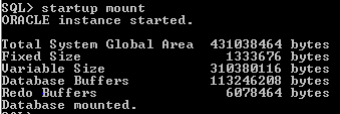
\includegraphics[width=14cm]{./Imagenes/imagen62} 
	\end{center}
  \\
    \\- STARTUP NOMOUNT:
    \\La instancia de base de datos está latente en memoria, con los procesos comunes funcionando. 
    \\Se abre el archivo de parámetros, se asigna en memoria el espacio para la SGA, 
    se lanzan los procesos en segundo plano, se abren los archivos de traza y alerta.
    \\
    \\- STARTUP FORCE:
    \\Hace SHUTDOWN ABORT y arranca la BD.
    \\
    \\- STARTUP RESTRICT:
    \\Es un modo especial de trabajo en el que la base de datos está abierta, pero solo se permite el acceso a usuarios 
    con permiso RESTRICTED (lo poseen los administradores) para hacer tareas especiales de administración.
    \\
    \\- STARTUP RECOVER:
    \\Especifica que la recuperación de medios se debe realizar, si es necesario, antes de iniciar la instancia. STARTUP RECOVER tiene el mismo efecto que emitir el comando RECOVER DATABASE e iniciar una instancia. Solo la recuperación completa es posible con la RECOVER option.
    \\
    \\- SHUTDOWN NORMAL:
    \\Espera a que terminen todas las transacciones en curso y todas las sesiones, 
    fuerza un checkpoint, además de cerrar todos los ficheros y destruir (parar) la instancia.
    \\
    \\- SHUTDOWN TRANSACTIONAL:
    \\Sólo espera a que terminen las transacciones en curso, fuerza un checkpoint, cierra los ficheros y destruye (para) la instancia.
    \\
    \\- SHUTDOWN ABORT:
     \\Cierra la instancia (destruye procesos background y SGA) sin esperar a desmontar ni cerrar la BD (como en una “caída”, ni hace checkpoint ni cierra ficheros). Requiere recovery de la instancia al arrancar (lo hace automáticamente el proceso SMON).

   \\- SHUTDOWN INMEDIATE:
   \\Hace rollback de todas las transacciones en curso y cierra todas las sesiones; cierra y desmonta la BD, además de forzar un checkpoint, cerrar ficheros y parar la instancia (como los anteriores).
   \\
   \item En el script lab-02-01.sql, se establecen privilegios de sistema, enliste los privilegios de sistema (DDL) 
   utilizados y describa cada uno de ellos.
   \\

   \item Enliste y describa los tipos de TableSpace que existen en Oracle.
   \\TIPOS DE TableSpace:
   \\- Tablespace SYSTEM.-
   \\*Se crea automáticamente al hacer la instalación de Oracle, o al crear una BD.
   \\*Contiene el diccionario de datos.
   \\
   \\- Tablespaces TEMPORALES.-
   \\*Es aquél en el que solamente puede haber objetos temporales. No se pueden crear objetos permanentes como pueden ser los índices, las tablas o los segmentos de rollback -> Optimización operaciones deordenación.
   \\*De tipo deshacer cambios.
   \\*Con tamaño de bloque variable.
   \\*De tipo BigFile.
   \\*De tipo SmallFile.
   \\
   \\- Tablespaces READ ONLY.-
   \\*Se pueden consultar los datos de los objetos, no se puede ni borrar niinsertar nada en ellos.
   \\*La principal ventaja de un tablespace read only es que no hace faltahacer backup del mismo.
   \\
   \\-Tablespaces SYSTEM Y SYSAUX.-
   \\Los tablespaces SYSTEM y SYSAUX son los únicos que, como mínimo, secrean con la BD (create database).
   \\*El tablespace SYSTEM (No debe contener datos de aplicaciones):
   \\*Contiene el DD, incluidos procedimientos almacenados, funciones,triggers y paquetes.
   \\*También alberga al segmento de rollback system.
   \\*El tablespace SYSAUX (>=10g) permite que en el tablespace SYSTEMsólo esté el DD, aglutinando las utilidades del sistema (Repositorio OEM,Intermedia, Spatial, OLAP, RMAN, XML DB, etc).
 \\
 \end{itemize}



\section{Crear Maquina Virtual}

	\begin{center}
\item PASOS DE CREACIÓN  DE  UNA MAQUINA VIRTUAL EN VMWARE WORKSTATION 14 

    \end{center}
    
\end{itemize}


\begin{itemize}
\item PASO 1:
\\Una vez abierto el VMWare Workstation 14 hacemos clic en Crear una máquina virtual
		\begin{center}
		\includegraphics[width=15cm]{./Imagenes/1}
		\end{center}
	

	\end{itemize} 
	

	\begin{itemize}
\item PASO 2:
\\Seleccionamos la última opción avanzada y clic en Next.
		\begin{center}
		\includegraphics[width=15cm]{./Imagenes/2}
		\end{center}
	

	\end{itemize} 
	
	\begin{itemize}
\item PASO 3:
\\Hacemos clic en Next sin hacer ninguna configuración.
		\begin{center}
		\includegraphics[width=15cm]{./Imagenes/3}
		\end{center}
	

	\end{itemize} 
	
	\begin{itemize}
\item PASO 4:
\\Seleccionamos la última opción  porque aún no tenemos el instalador y clic en Next
		\begin{center}
		\includegraphics[width=15cm]{./Imagenes/4}
		\end{center}
		\\\
	\end{itemize} 
	
	
	\begin{itemize}

\item PASO 5:
\\Seleccionamos  el tipo de sistema operativo Linux y la versión CentOS 6 y clic en Next.
		\begin{center}
		\includegraphics[width=15cm]{./Imagenes/5}
		\end{center}
	

	\end{itemize} 

	\begin{itemize}
\item PASO 6:
\\Escribimos un nombre y fijamos la dirección de la máquina virtual y clic en Next.
		\begin{center}
		\includegraphics[width=15cm]{./Imagenes/6}
		\end{center}
		\\\

	\end{itemize} 

	\begin{itemize}
\item PASO 7:
\\Colocamos 1 GB de memoria RAM como mínimo y clic en Next.
		\begin{center}
		\includegraphics[width=15cm]{./Imagenes/7}
		\end{center}
	

	\end{itemize} 

	\begin{itemize}
\item PASO 8:
\\Seleccionamos la tarjeta de red en este caso bridged networking y clic en Next.
		\begin{center}
		\includegraphics[width=15cm]{./Imagenes/8}
		\end{center}
	

	\end{itemize} 

	\begin{itemize}
\item PASO 9:
\\Lo dejamos seleccionado en LSI Logic (Recommended) y clic en Next.
		\begin{center}
		\includegraphics[width=15cm]{./Imagenes/9}
		\end{center}
	

	\end{itemize} 

	\begin{itemize}
\item PASO 10:
\\Seleccionamos SCSI (Recommended) y clic en Next.
		\begin{center}
		\includegraphics[width=15cm]{./Imagenes/10}
		\end{center}
	

	\end{itemize} 

	\begin{itemize}
\item PASO 11:
\\Seleccionar la primera opción donde crearemos una nueva máquina virtual y clic en Next.\\
		\begin{center}
		\includegraphics[width=15cm]{./Imagenes/11}
		\end{center}
	

	\end{itemize} 

	\begin{itemize}
\item PASO 12:
\\Definimos el tamaño de disco en este caso es 60 GB y clic en Next.\\
		\begin{center}
		\includegraphics[width=15cm]{./Imagenes/12}
		\end{center}
	

	\end{itemize} 

	\begin{itemize}
\item PASO 13:
\\Una vez terminado nos va a mostrar un resumen de las características de la nueva máquina virtual CentOS 6.2 y clic en Finish.
\\
		\begin{center}
		\includegraphics[width=15cm]{./Imagenes/13}
		\end{center}
	

	\end{itemize} 

	\begin{itemize}
\item PASO 14:
\\Finalmente tenemos nuestra máquina virtual creada y sus características.\\
		\begin{center}
		\includegraphics[width=15cm]{./Imagenes/14}
		\end{center}
	

	\end{itemize} 



\begin{itemize}


  \end{itemize}
  
  



\end{document}
